% Detaljer hur styrenheten är designad

\section{Styrenhet}

Styrenheten har till uppgift att ta kommandon från huvudenheten och producera utsignaler som motorer och servon kan förstå.

\subsection{Hårdvara}
Styrenheten består av en Atmega1284p, en tri-state-krets\cite{tristate}, två motorpar och en robotarm Trossenrobotics Reactor\cite{robotarm}. Styrenheten är ansluten till Huvudenheten via samma \todo{20lol-pinnarskabel} som Sensorenheten. Figur \ref{styr-oversikt} illustrerar grovt hur de är ihopkopplade. \todo{Hänvisa till kopplingsschema i Bilaga}

\begin{figure}[h!]
	\centering
	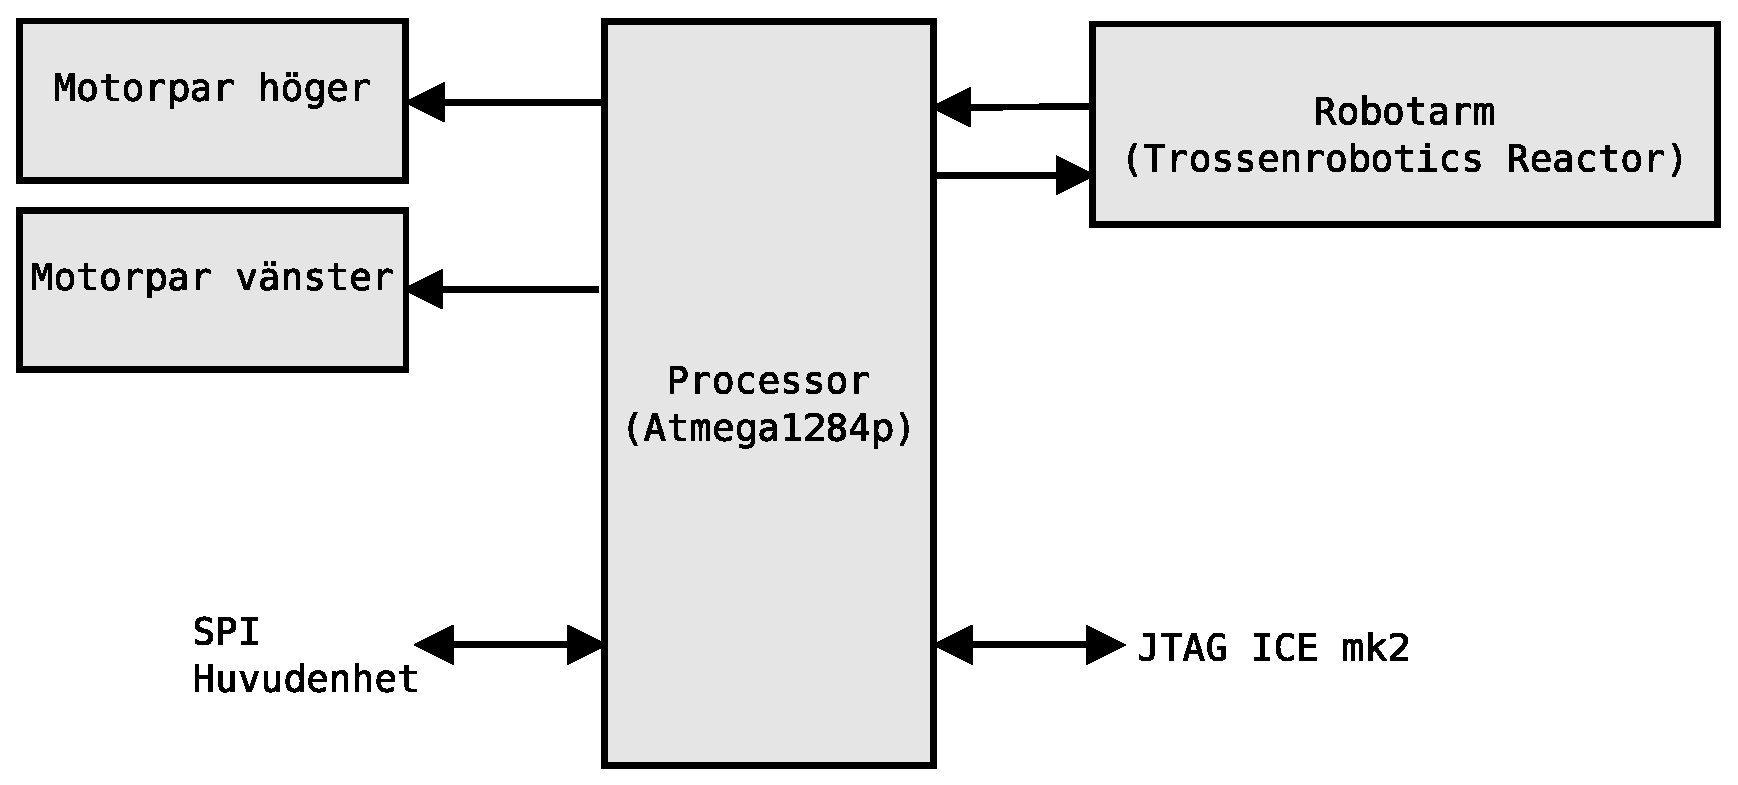
\includegraphics[scale=0.4]{grafik/styrenhet-oversikt}
	\caption{Översikt av styrenheten} \label{styr-oversikt}
\end{figure}

\subsubsection{Motorer}
Systemet har sammanlagt fyra motorer, uppdelat i två motorpar. De är anslutna till Styrenheten med en 10-pinnars flatkabel. Motorparen levererades med intelligenta H-bryggor\cite{pwmmotor} och behöver förses med en PWM-signal var, som bestämmer motorernas hastighet och en riktningssignal var där $1$ är i framriktningen och $0$ backriktningen \todo{Stämmer?}.

\subsubsection{Robotarm}
Robotarmen är en Trossenrobotics Reactor och består av åtta servon av typ AX-12a\cite{servo}. Dessa är fördelade på fem axlar och en gripklo. De kommunicerar med Styrenheten över UART med en baudrate på 1MB/s, där både in och utsignal går via samma sladd. Denna är därför ansluten till två tristates för att förebygga att något oväntat skrivs eller läses från bussen.

\todo{Utveckla hur protokollet mot armen ser ut?}

\subsubsection{Processor}
Styrenheten drivs av en enkretsdator av typ Atmega1284p. Den kan anslutas till en PC via JTAG för att programmeras eller felsökas. Den har en klockfrekvens på 16MHz och tar emot kommandon från Huvudenheten, tolkar dessa och ser till att motorerna och robotarmen utför det som Huvudenheten har sagt. Figur \ref{styr-processor} visar hur enkretsdatorn är ansluten till övrig hårdvara.

\begin{figure}[h!]
	\centering
	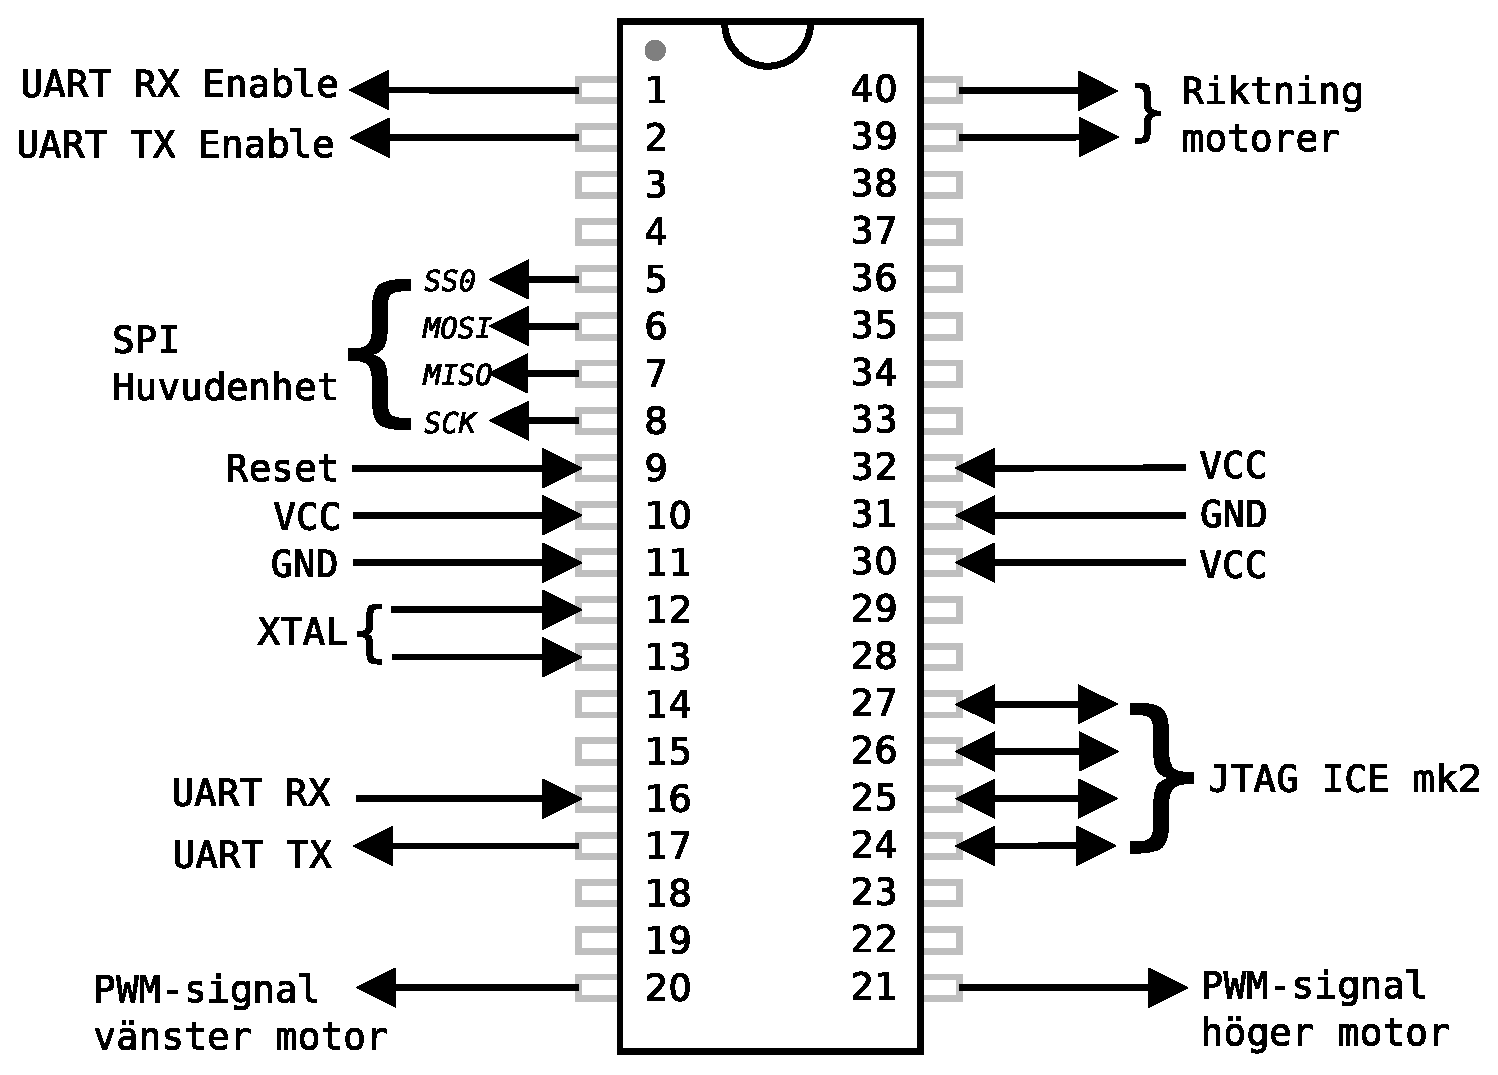
\includegraphics[scale=0.5]{grafik/styrenhet-processor}
	\caption{Schema över hur enkretssdatorn i styrenheten är ansluten till övrig hårdvara.} \label{styr-processor}
\end{figure}

\subsection{Mjukvara}
\todo{Hur sköts PWM-en?}
\todo{Hur kommunicerar vi med Armen? Hårdvarustöd UART}
\todo{Hur tar vi emot kommandon från Huvudenheten?}
\todo{Flödesschema styrenheten}
